\documentclass[13pt,a4]{article}
\usepackage{sbc-template}
\usepackage{listings}
\usepackage[brazil]{babel} 
\usepackage[utf8]{inputenc}  
\usepackage[T1]{fontenc}  
\usepackage{tabularx}
\usepackage{indentfirst}
\usepackage{graphicx}
\usepackage{url}
\usepackage{float} 
\usepackage{color}

\definecolor{dkgreen}{rgb}{0,0.6,0}
\definecolor{gray}{rgb}{0.5,0.5,0.5}
\definecolor{mauve}{rgb}{0.58,0,0.82}
\definecolor{darkblue}{rgb}{0.0,0.0,0.6}
\definecolor{cyan}{rgb}{0.0,0.6,0.6}
\definecolor{mygray}{rgb}{0.47,0.47,0.33}
\definecolor{myorange}{rgb}{0.8,0.4,0}
\definecolor{mywhite}{rgb}{0.98,0.98,0.98}
\definecolor{myblue}{rgb}{0.01,0.61,0.98}

\lstset{
	backgroundcolor=\color{mywhite},   
	basicstyle=\footnotesize,       
	breakatwhitespace=false,         
	breaklines=true,                 
	captionpos=b,                   
	commentstyle=\color{dkgreen},    
	deletekeywords={...},           
	escapeinside={\%*}{*)},          
	extendedchars=true,              
	frame=shadowbox,                    
	keepspaces=true,                 
	keywordstyle=\color{myorange},       
	language=Octave,                
	morekeywords={*,...},            
	numbers=left,                    
	numbersep=5pt,                   
	numberstyle=\tiny\color{mygray}, 
	rulecolor=\color{black},         
	showspaces=false,                
	showstringspaces=false,          
	showtabs=false,                  
	stepnumber=2,                    
	stringstyle=\color{myorange},    
	tabsize=2,                       
	title=\lstname                   
}

\newcommand{\aspas}[1]{``#1''}
\newcommand{\ident}{\hspace*{0.5cm}}

\hyphenation{ar-ma-ze-ná-los}
   
\sloppy

\title{Tutorial - Segurança residencial utilizando Arduino, sensores de presença PIR, finger print e shield ethernet   }
\author{Bruno Tomé, Cláudio Menezes }

\address{Departamento de Ciência da Computação\\
Instituto Federal de Minas Gerais,Campus Formiga (IFMG)\\Formiga, MG -- Brasil
   \email{ibrunotome@gmail.com, claudiomenezio@gmail.com}
}

\begin{document} 

\maketitle

\begin{resumo}
	 Neste tutorial é demonstrado como interligar o Arduino com os shield's PIR, ethernet e fingerprint. Bem como a interação do Arduino com os shield's e suas bibliotecas. Como projeto final temos a união destes componentes para um sistema de segurança residencial.
\end{resumo}

\section{Introdução }
     Neste tutorial será apresentado o passo a passo de como fazer as ligações entre o Arduino, \textit{protoboard} e \textit{shield's}. Em seguida mostraremos o código utilizado em cada \textit{shield} e como resultado final temos um protótipo de sistema de segurança residencial que utiliza sensores PIR, sensor \textit{fingerprint} e um \textit{shield ethernet} para enviar as informações de presença para um servidor web, que envia \textit{emails} ao dono da residência informando o local da movimentação.

\subsection{Módulo Ethernet}
	O \textit{shield ethernet} é simplesmente acoplado em cima do Arduino. Com o \textit{software} \textit{Arduino} aberto, vá em \textit{File/Examples/Ethernet/WebClient} que serve como um cliente que envia informações ao servidor. 

\begin{figure}[!htb]
	\centering
	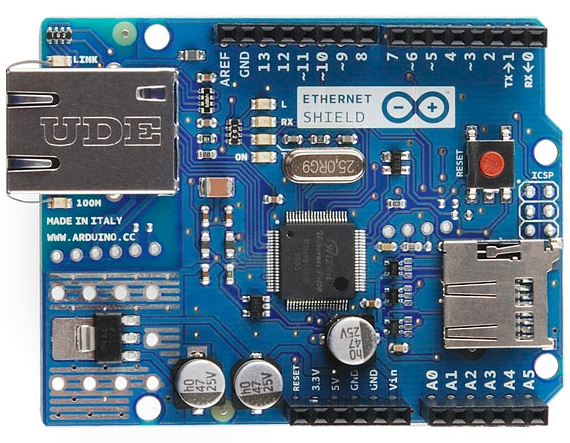
\includegraphics[scale=0.35]{etherPin.jpg}
	\caption{ Decodificador para o display de 7 segmentos	}
	\label{}
\end{figure}

\section{Sensor de Presença - PIR} 	

	Na figura abaixo podemos ver como fazer a pinagem do sensor de presença PIR. São somente três saídas, uma saída para \textit{ GND, VCC} e um \textit{OUTPUT} para passar as informações lidas: 
\begin{figure}[!htb]
	\centering
	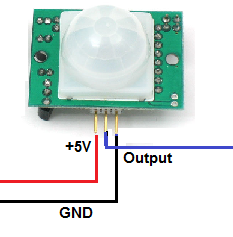
\includegraphics[scale=0.55]{PIRpin.png}
	\caption{ Descrição da pinagem sensor PIR	}
	\label{}
\end{figure}

	Em seguida é realizado as ligações das três saídas do sensor \textit{PIR} no Arduino. A saída da esquerda é ligada a entrada de \textit{5V} e a da direta é ligada ao \textit{GND}, do arduino. O \textit{OUTPUT} que é a saída do meio do sensor é conectada ao pino número 2 do Arduino, como mostrado na figura abaixo:

\begin{figure}[!htb]
	\centering
	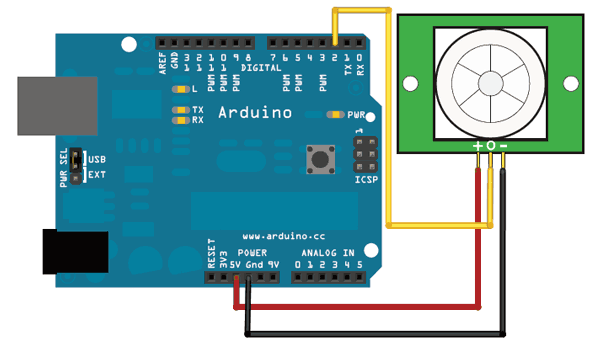
\includegraphics[scale=0.45]{pir2.png}
	\caption{Sensor PIR ligado ao Arduino}
	\label{}
\end{figure}

\subsection{Código sensor PIR}
 	O código abaixo exibe no monitor serial a frase \textit{Movimento detectado} quando o sensor é acionado: 
 
 \lstinputlisting[language = c, showstringspaces=false, columns=flexible, stringstyle=\color{mauve}, tabsize=4, caption=Código fonte para o Sensor de presença PIR]{pirCodigo.ino}
 
\section{Leitor Biométrico - Finger Print}

	A figura abaixo mostra a pinagem para o leitor biométrico, contendo quatro saídas, sendo duas para \textit{ GND, VCC} e outras duas, uma para \textit{RX(Data IN)} e a outra \textit{TX(Data OUT)} para passar as informações lidas no módulo: 

\begin{figure}[!htb]
	\centering
	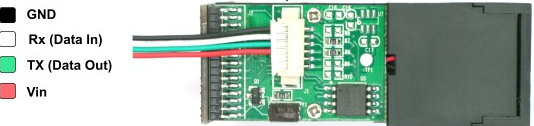
\includegraphics[scale=0.50]{fingerPin.png}
	\caption{  Descrição da pinagem para o leitor biométrico}
	\label{}
\end{figure}

	A próxima figura mostra como é realizada  a ligação das saídas do Leitor Biométrico  no Arduino. As saídas em vermelho e preto são ligadas no Arduino em \textit{5V} e \textit{GND} respectivamente. As duas saídas  restantes são a \textit{RX} em amarelo e em vermelho a \textit{TX}, respectivamente ligadas nos pinos do Arduino  \textit{RX e TX}.

\begin{figure}[!htb]
	\centering
	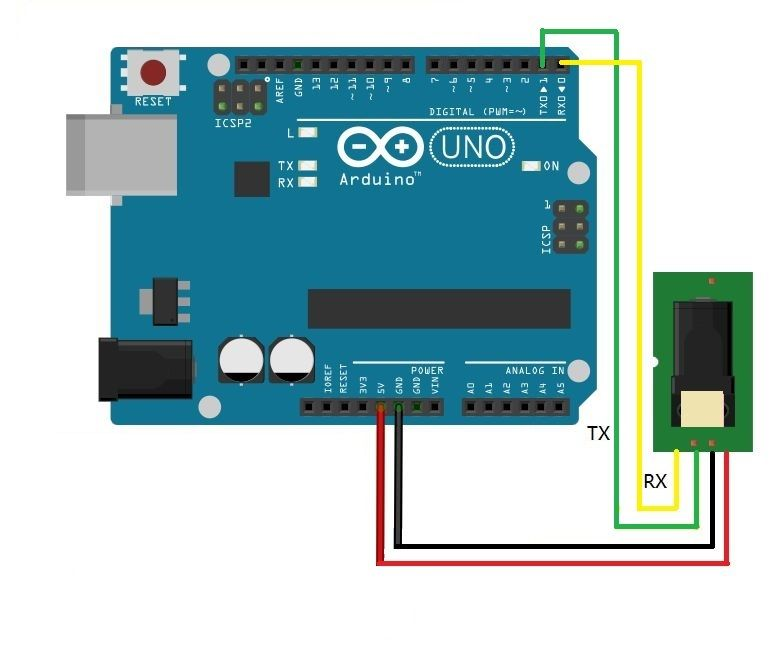
\includegraphics[scale=0.40]{finger2.jpg}
	\caption{ Leitor biométrico ligado ao Arduino	}
	\label{}
\end{figure}
 
\subsection{Código} 
	 Inicialmente para trabalhar com o leitor deve-se baixar a biblioteca \textit{Adafruit library} disponível neste link: \textit{https://github.com/adafruit/Adafruit-Fingerprint-Sensor-Library} e colocá-la na pasta de bibliotecas do Arduino. 
	 	
	 Podemos entender como é feito o ato de gravar uma digital no módulo. Com o software \textit{Arduino} aberto, vá em \textit{File/Examples/Adafruit Fingerprint Sensor Library/enroll} 
	 
	 Um exemplo de código que mostra como é feito o \textit{match} entre uma digital já cadastrada no módulo e uma recém inserida no módulo pode ser visto com o software \textit{Arduino} aberto, vá em \textit{File/Examples/Adafruit Fingerprint Sensor Library/fingerprint}.
 
\section{Projeto Desenvolvido}

O projeto desenvolvido é um protótipo de sistema de segurança residencial que utiliza sensores PIR, sensor \textit{fingerprint} e um \textit{shield ethernet} para enviar as informações de presença para um servidor \textit{web}, que envia \textit{emails} ao dono da residência informando o local da movimentação.

O sistema requere a autenticação da digital para começar a funcionar e assim que ativado, os sensores PIR começam a captar os movimentos e enviar \textit{POSTS} ao servidor contendo informações de quem está enviado, o que está acontecendo e em qual cômodo da residência está acontecendo. Para desativar o sistema, basta autenticar com a digital novamente.
 
\subsection{Materiais Utilizados}
	\begin{itemize}
		\item Um Arduino UNO 
		\item Um shield Ethernet W5100
		\item Um  Leitor Biométrico De Impressão Digital
		\item Quatro sensores de infra vermelho por temperatura (PIR)
		\item Protoboard
	\end{itemize}
 
\subsection{Código Arduino} 

Abaixo está listado o código utilizado no Arduino para realização do projeto.
\lstinputlisting[language=c, showstringspaces=false, columns=flexible, stringstyle=\color{mauve}, tabsize=4, caption=Código fonte do projeto]{../Projeto.ino}

\subsection{Web}

O protótipo contou com uma interface \textit{web} para analisar a situação atual da residência e também com o envio de emails para o dono da mesma. Assim que o usuário realiza o \textit{login} no sistema ele vê a atualização mais recente sobre sua residência e tem acesso a um menu listando todos os alertas feitos até o momento com suas respectivas datas.

A figura 6 abaixo mostra a interface web criada para o projeto.

\newpage

\begin{figure}[!htb]
	\centering
	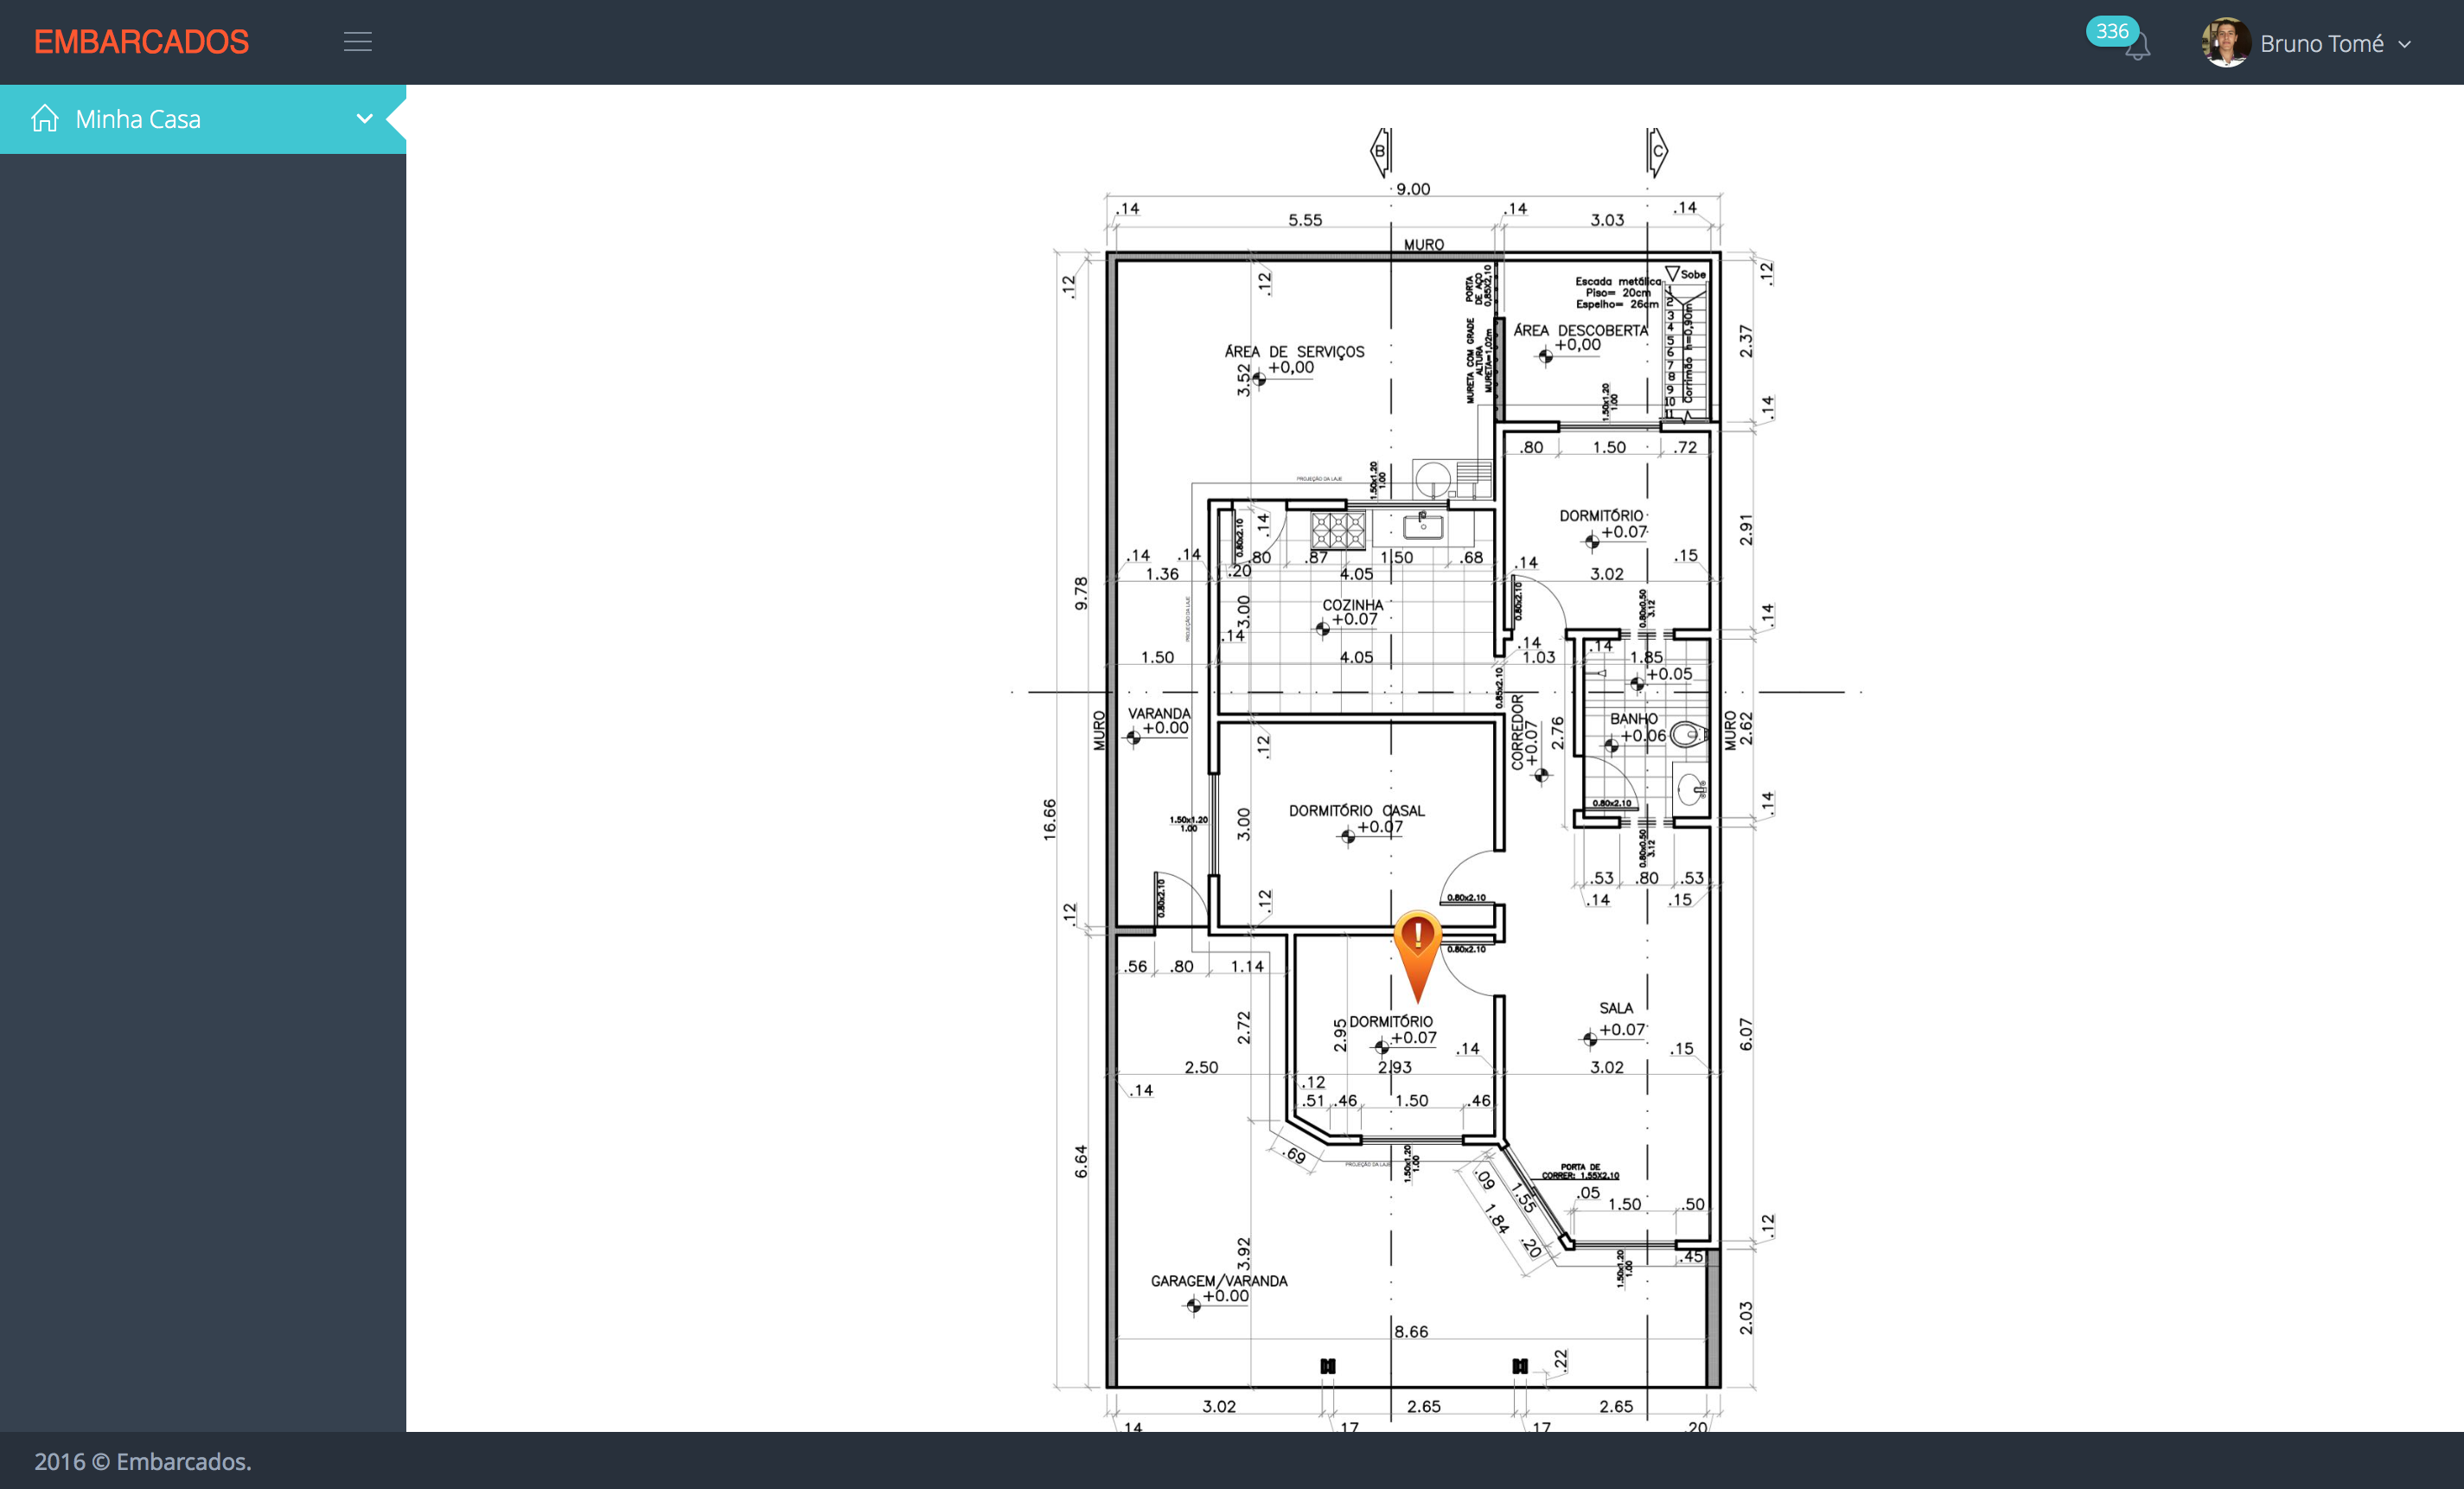
\includegraphics[scale=0.30]{web.png}
	\caption{Interface web para controle dos alertas recebidos}
	\label{}
\end{figure}

A figura 7 mostra um exemplo de email recebido pelo dono da residência:

\begin{figure}[!htb]
	\centering
	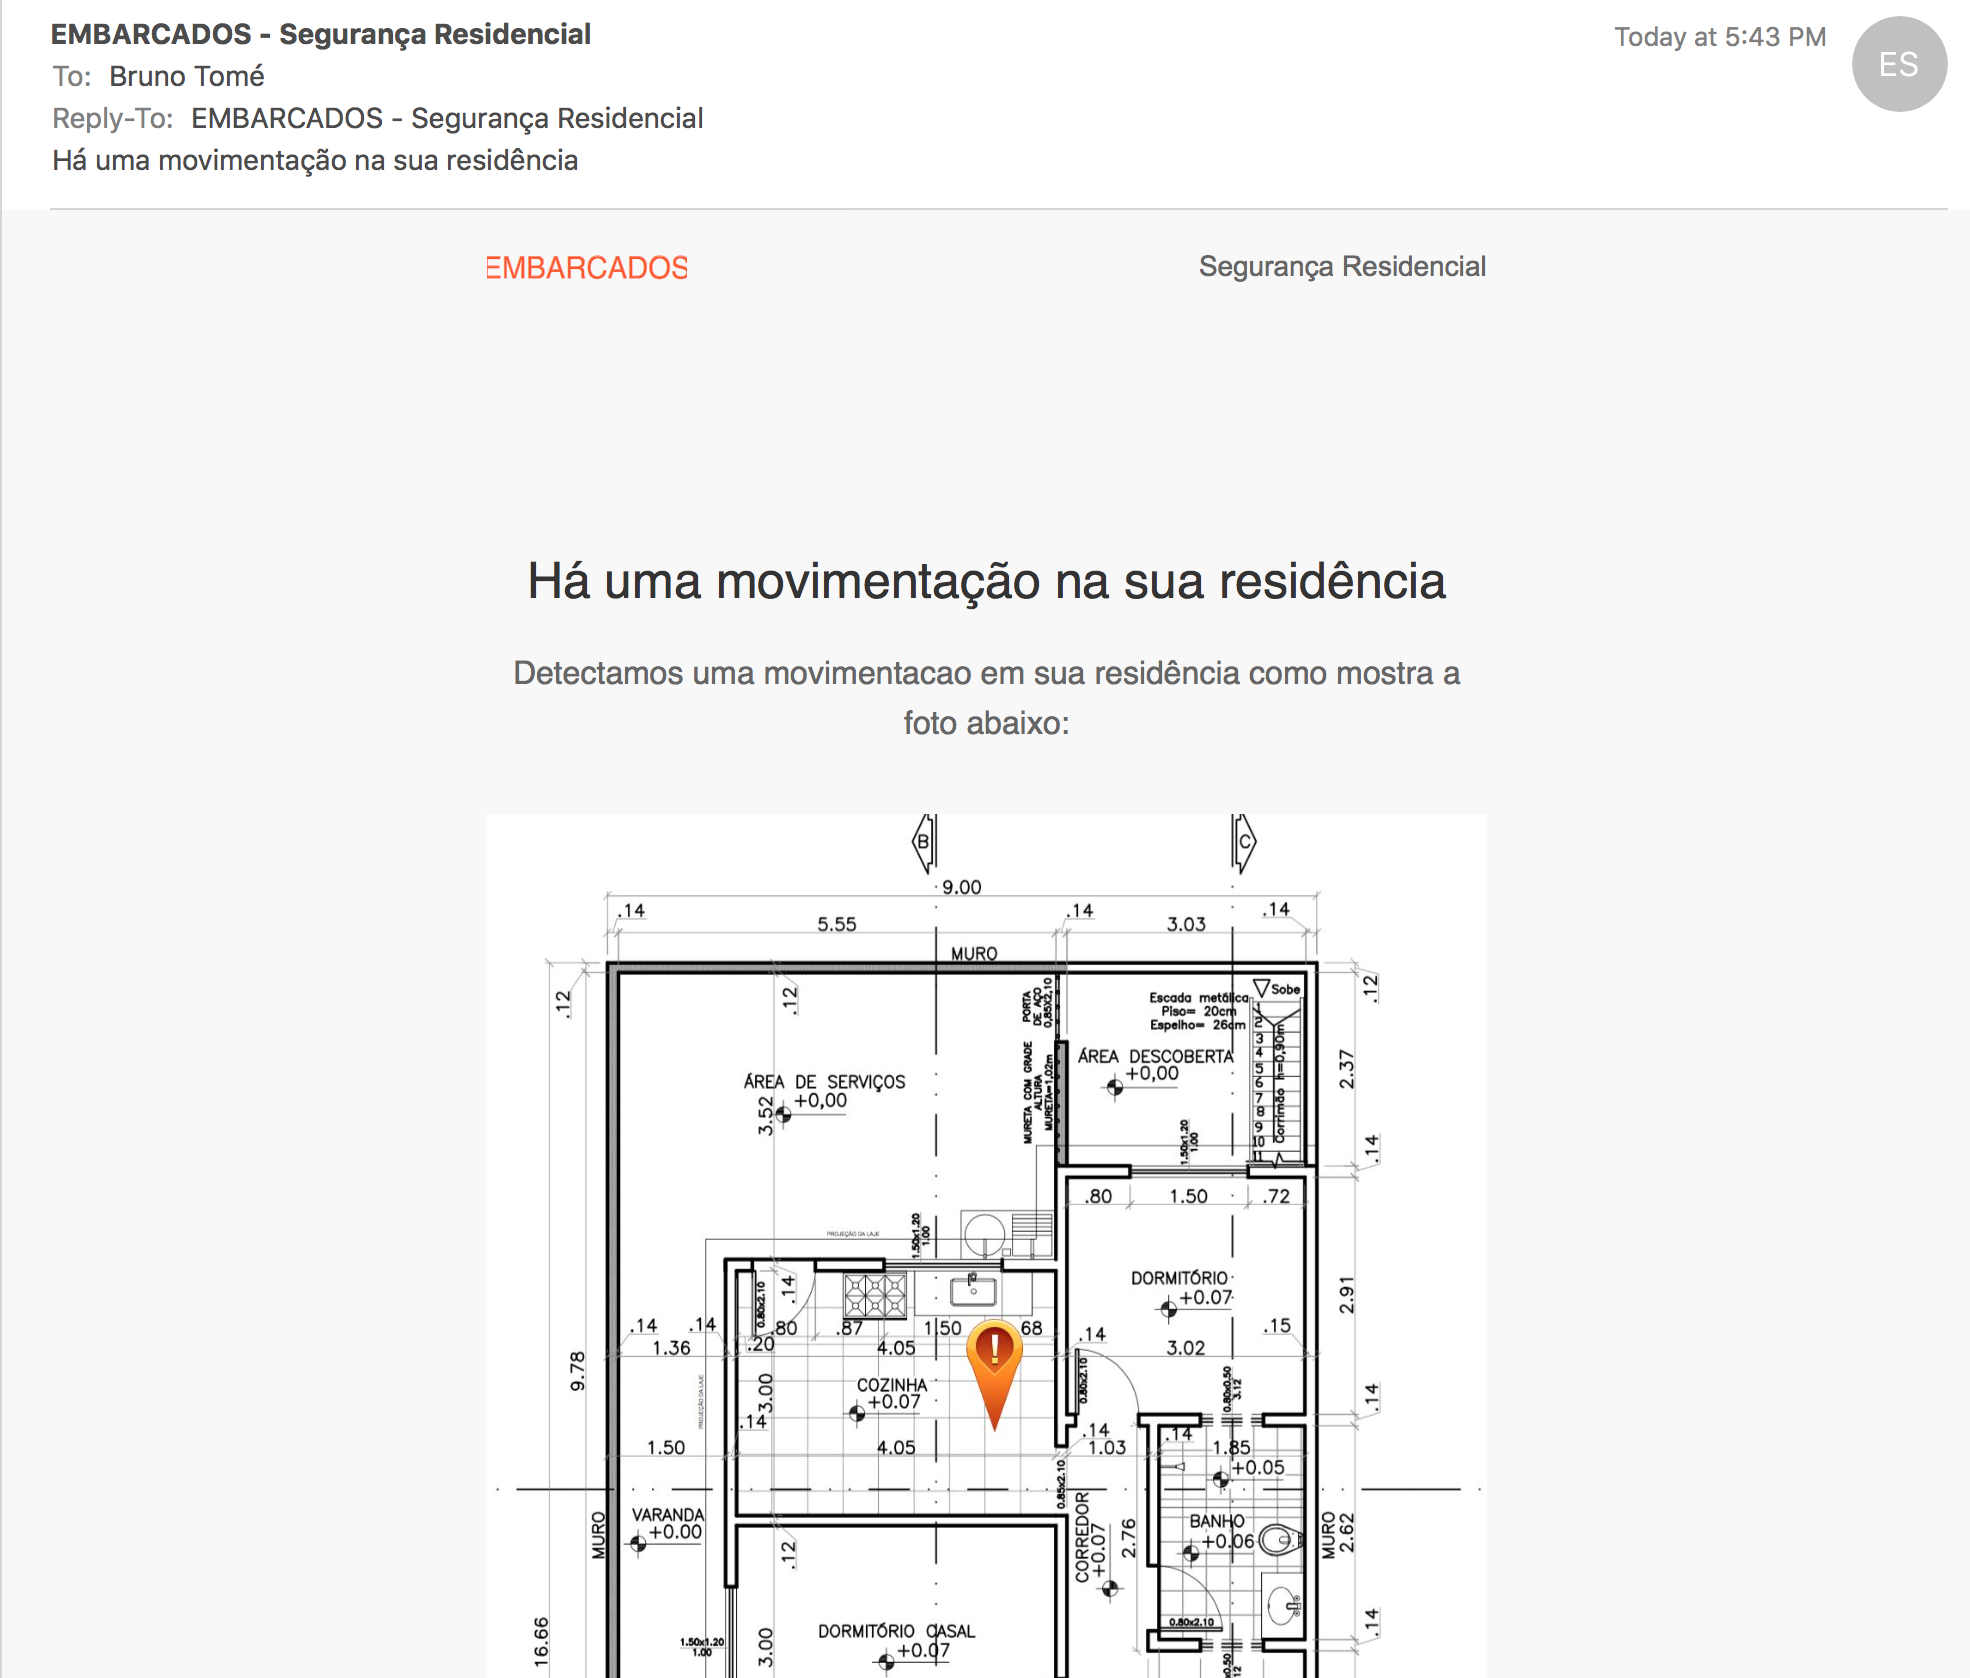
\includegraphics[scale=0.30]{email.png}
	\caption{Exemplo de email recebido pelo dono da residência}
	\label{}
\end{figure}

\subsubsection{Código PHP}

Abaixo está listado o código PHP que recebe os posts enviados pelo Arduino, armazena tais informações e envia emails ao proprietário da residência quando necessário.

\lstinputlisting[language=php, showstringspaces=false, columns=flexible, stringstyle=\color{mauve}, tabsize=4, caption=Código fonte do projeto]{update.php}

\subsection{Resultado final}

Abaixo na figura 8, o circuito do protótipo final do sistema de segurança residencial.

\begin{figure}[!htb]
	\centering
	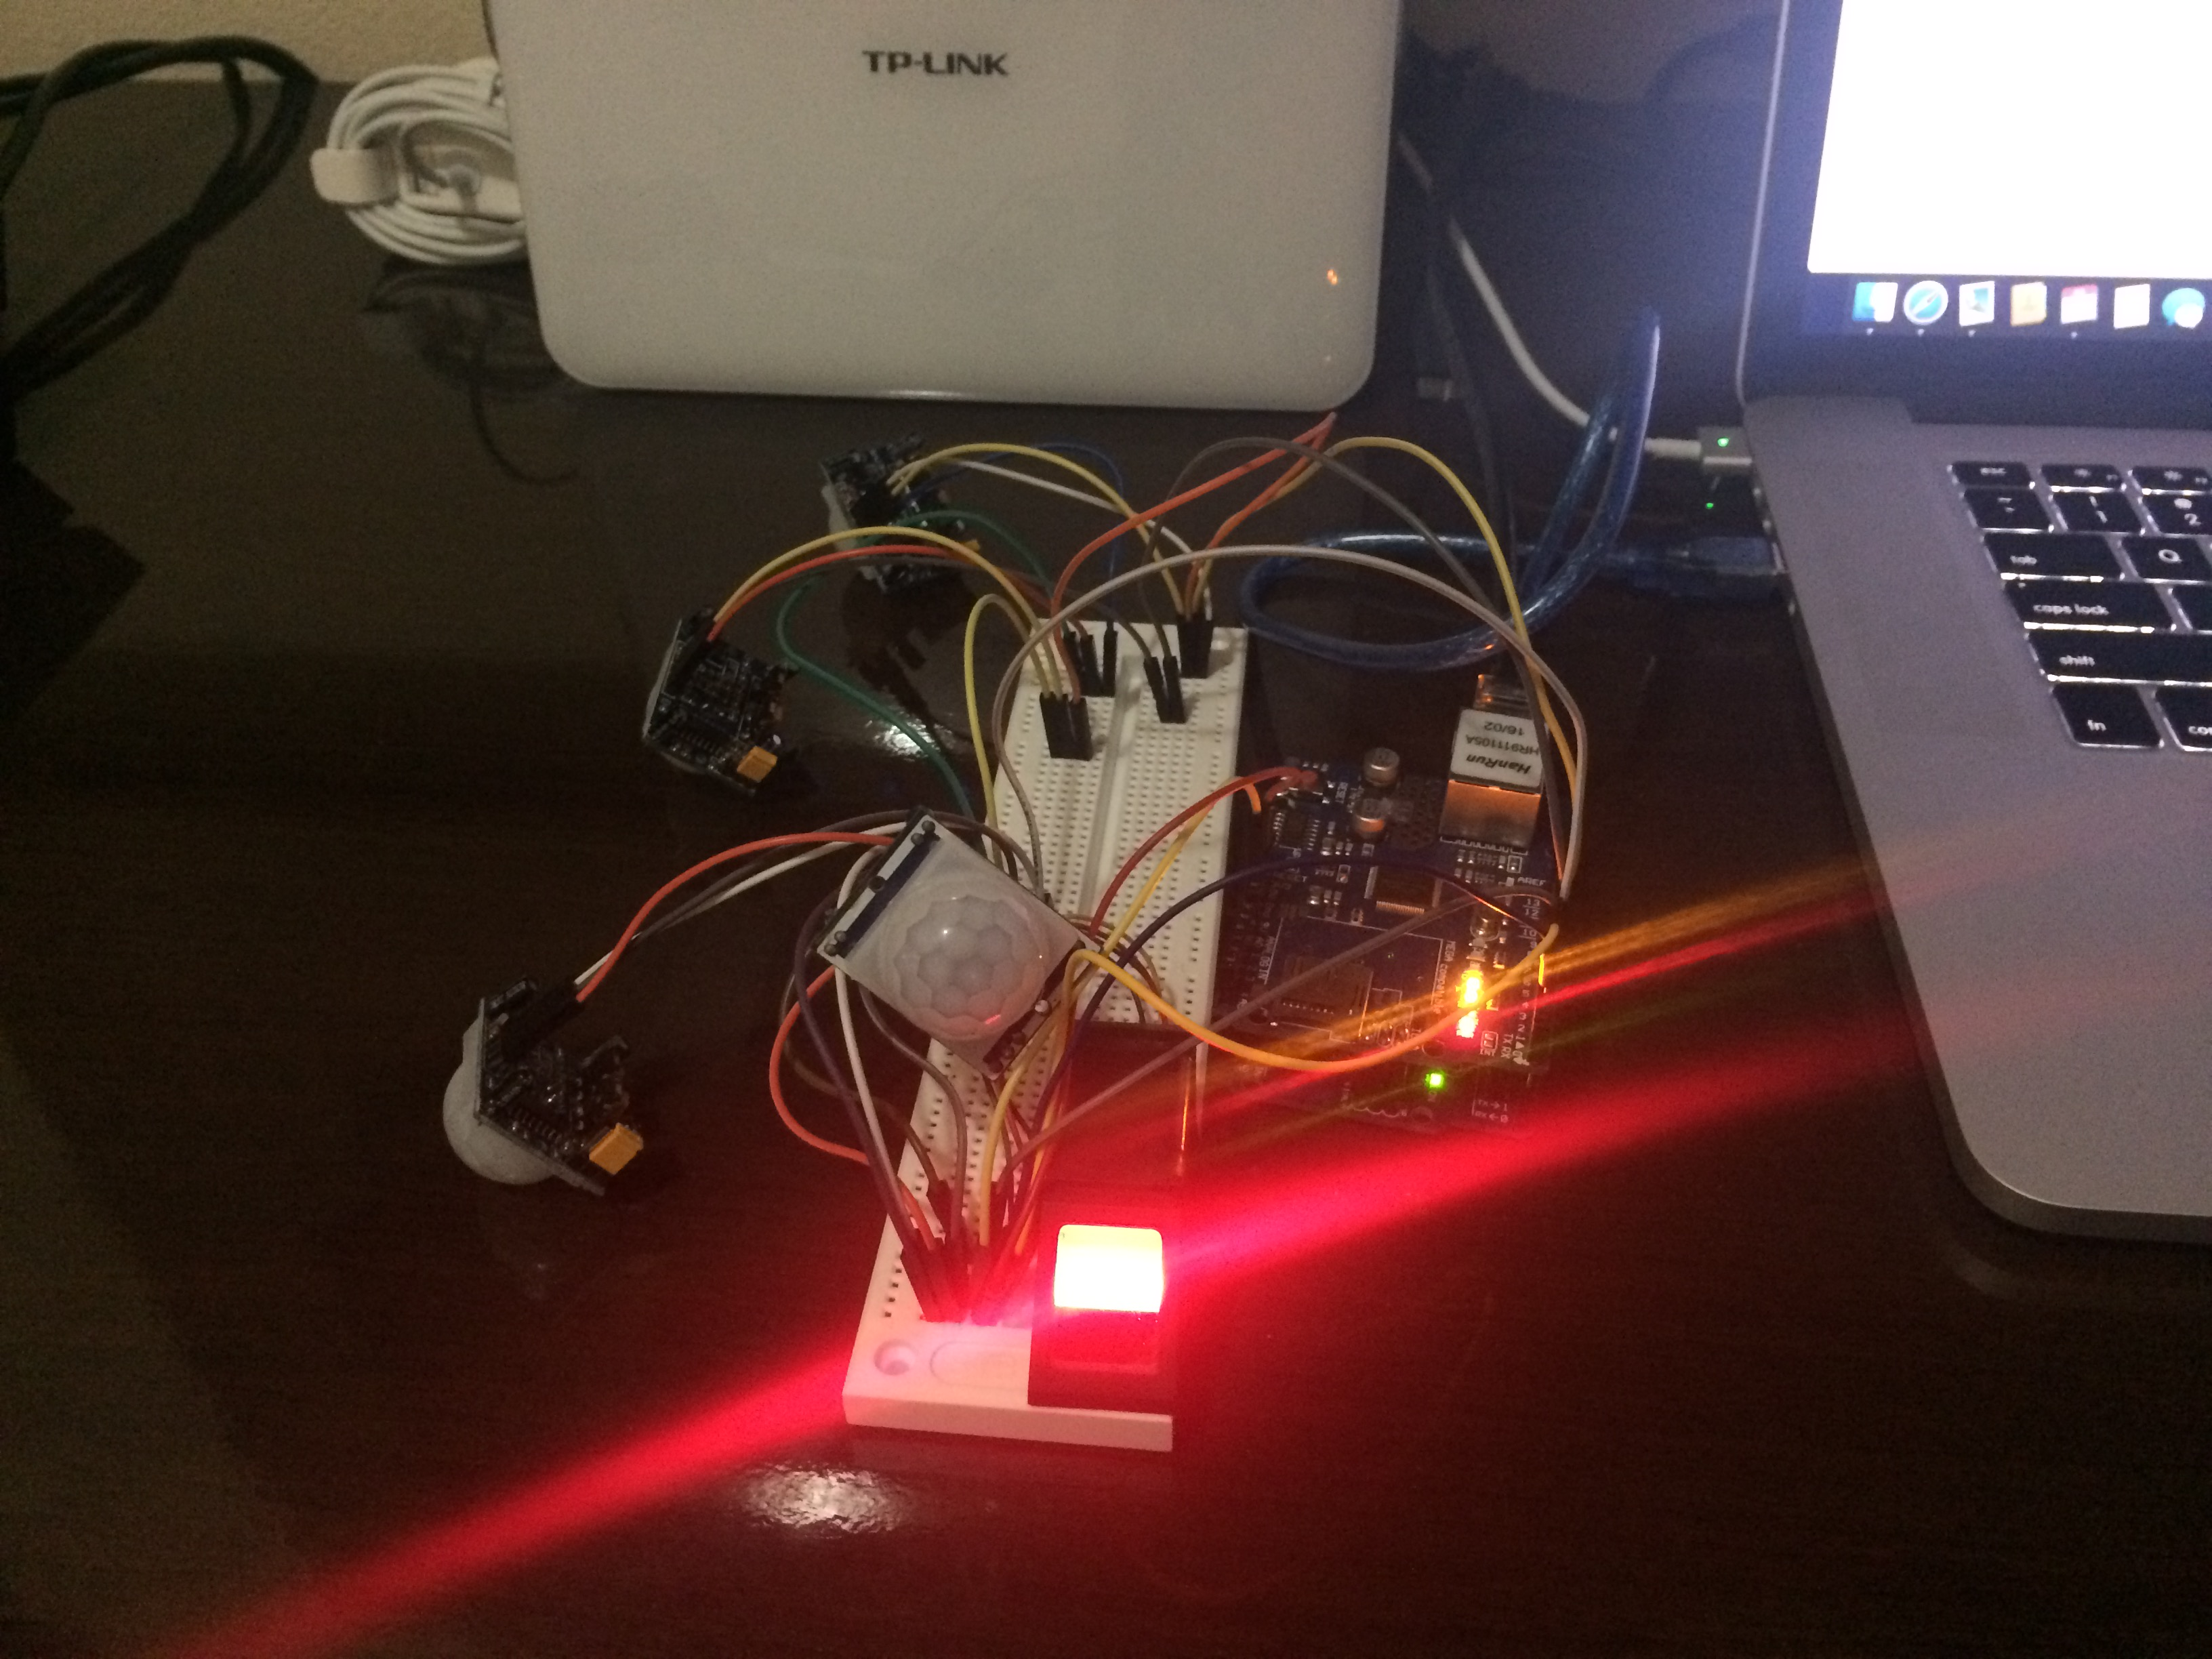
\includegraphics[scale=0.1]{final.jpg}
	\caption{Exemplo de email recebido pelo dono da residência}
	\label{}
\end{figure}

\section{Bibliografia}

Getting Started with the Arduino Ethernet Shield. Disponível em: <https://www.arduino.cc/en/Guide/ArduinoEthernetShield>
 
Manual Adafruit Optical Fingerprint Sensor

Tutorial: como utilizar o Sensor PIR (Passive Infrared) com Arduino. Disponível em: <http://labdegaragem.com/profiles/blogs/tutorial-emissor-e-receptor-infra-vermelho-com-arduino>
   
\end{document}
